\documentclass[10pt,a4paper,onecolumn]{article}
\usepackage{marginnote}
\usepackage{graphicx}
\usepackage[rgb,svgnames]{xcolor}
\usepackage{authblk,etoolbox}
\usepackage{titlesec}
\usepackage{calc}
\usepackage{tikz}
\usepackage[pdfa]{hyperref}
\usepackage{hyperxmp}
\hypersetup{%
    unicode=true,
    pdfapart=3,
    pdfaconformance=B,
    pdftitle={Article Writing with Markdown and the Open Journals
publishing pipeline},
    pdfauthor={Albert Krewinkel, Juanjo Bazán, Arfon M. Smith},
    pdfpublication={Journal of Open Source Software},
    pdfpublisher={Open Journals},
    pdfissn={2475-9066},
    pdfpubtype={journal},
    pdfvolumenum={},
    pdfissuenum={},
    pdfdoi={N/A},
    pdfcopyright={Copyright (c) 1970, Albert Krewinkel, Juanjo Bazán,
Arfon M. Smith},
    pdflicenseurl={http://creativecommons.org/licenses/by/4.0/},
    colorlinks=true,
    linkcolor=[rgb]{0.0, 0.5, 1.0},
    citecolor=Blue,
    urlcolor=[rgb]{0.0, 0.5, 1.0},
    breaklinks=true
}
% https://tex.stackexchange.com/a/535849
% Create an OutputIntent in order to correctly specify colours
\immediate\pdfobj stream attr{/N 3} file{sRGB.icc}
\pdfcatalog{%
  /OutputIntents [
    <<
      /Type /OutputIntent
      /S /GTS_PDFA1
      /DestOutputProfile \the\pdflastobj\space 0 R
      /OutputConditionIdentifier (sRGB)
      /Info (sRGB)
    >>
  ]
}
\pdfvariable omitcidset=1
\usepackage{caption}
\usepackage{orcidlink}
\usepackage{tcolorbox}
\usepackage{amssymb,amsmath}
\usepackage{ifxetex,ifluatex}
\usepackage{seqsplit}
\usepackage{xstring}

\usepackage{float}
\let\origfigure\figure
\let\endorigfigure\endfigure
\renewenvironment{figure}[1][2] {
    \expandafter\origfigure\expandafter[H]
} {
    \endorigfigure
}

\usepackage{fixltx2e} % provides \textsubscript

% definitions for citeproc citations
\NewDocumentCommand\citeproctext{}{}
\NewDocumentCommand\citeproc{mm}{%
  \begingroup\def\citeproctext{#2}\cite{#1}\endgroup}
\makeatletter
 % allow citations to break across lines
 \let\@cite@ofmt\@firstofone
 % avoid brackets around text for \cite:
 \def\@biblabel#1{}
 \def\@cite#1#2{{#1\if@tempswa , #2\fi}}
\makeatother
\newlength{\cslhangindent}
\setlength{\cslhangindent}{1.5em}
\newlength{\csllabelwidth}
\setlength{\csllabelwidth}{3em}
\newenvironment{CSLReferences}[2] % #1 hanging-indent, #2 entry-spacing
 {\begin{list}{}{%
  \setlength{\itemindent}{0pt}
  \setlength{\leftmargin}{0pt}
  \setlength{\parsep}{0pt}
  % turn on hanging indent if param 1 is 1
  \ifodd #1
   \setlength{\leftmargin}{\cslhangindent}
   \setlength{\itemindent}{-1\cslhangindent}
  \fi
  % set entry spacing
  \setlength{\itemsep}{#2\baselineskip}}}
 {\end{list}}
\usepackage{calc}
\newcommand{\CSLBlock}[1]{\hfill\break\parbox[t]{\linewidth}{\strut\ignorespaces#1\strut}}
\newcommand{\CSLLeftMargin}[1]{\parbox[t]{\csllabelwidth}{\strut#1\strut}}
\newcommand{\CSLRightInline}[1]{\parbox[t]{\linewidth - \csllabelwidth}{\strut#1\strut}}
\newcommand{\CSLIndent}[1]{\hspace{\cslhangindent}#1}

% --- Page layout -------------------------------------------------------------
\usepackage[top=3.5cm, bottom=3cm, right=1.5cm, left=1.0cm,
            headheight=2.2cm, reversemp, includemp, marginparwidth=4.5cm]{geometry}

% --- Default font ------------------------------------------------------------
\renewcommand\familydefault{\sfdefault}

% --- Style -------------------------------------------------------------------
\renewcommand{\captionfont}{\small\sffamily}
\renewcommand{\captionlabelfont}{\bfseries}

% --- Section/SubSection/SubSubSection ----------------------------------------
\titleformat{\section}
  {\normalfont\sffamily\Large\bfseries}
  {}{0pt}{}
\titleformat{\subsection}
  {\normalfont\sffamily\large\bfseries}
  {}{0pt}{}
\titleformat{\subsubsection}
  {\normalfont\sffamily\bfseries}
  {}{0pt}{}
\titleformat*{\paragraph}
  {\sffamily\normalsize}


% --- Header / Footer ---------------------------------------------------------
\usepackage{fancyhdr}
\pagestyle{fancy}
\fancyhf{}
%\renewcommand{\headrulewidth}{0.50pt}
\renewcommand{\headrulewidth}{0pt}
\fancyhead[L]{\hspace{-0.75cm}
\includegraphics[width=5.5cm]{joss/logo.png}}
\fancyhead[C]{}
\fancyhead[R]{}
\renewcommand{\footrulewidth}{0.25pt}

\fancyfoot[L]{\parbox[t]{0.98\headwidth}{\footnotesize{\sffamily Krewinkel
et al. (1970). Article Writing with Markdown and the Open Journals
publishing pipeline. \emph{Journal of Open Source Software},
\emph{¿VOL?}(¿ISSUE?), ¿PAGE? \url{https://doi.org/N/A}}.}}


\fancyfoot[R]{\sffamily \thepage}
\makeatletter
\let\ps@plain\ps@fancy
\fancyheadoffset[L]{4.5cm}
\fancyfootoffset[L]{4.5cm}

% --- Macros ---------

\definecolor{linky}{rgb}{0.0, 0.5, 1.0}

\newtcolorbox{repobox}
   {colback=red, colframe=red!75!black,
     boxrule=0.5pt, arc=2pt, left=6pt, right=6pt, top=3pt, bottom=3pt}

\newcommand{\ExternalLink}{%
   \tikz[x=1.2ex, y=1.2ex, baseline=-0.05ex]{%
       \begin{scope}[x=1ex, y=1ex]
           \clip (-0.1,-0.1)
               --++ (-0, 1.2)
               --++ (0.6, 0)
               --++ (0, -0.6)
               --++ (0.6, 0)
               --++ (0, -1);
           \path[draw,
               line width = 0.5,
               rounded corners=0.5]
               (0,0) rectangle (1,1);
       \end{scope}
       \path[draw, line width = 0.5] (0.5, 0.5)
           -- (1, 1);
       \path[draw, line width = 0.5] (0.6, 1)
           -- (1, 1) -- (1, 0.6);
       }
   }

\definecolor{c53baa1}{RGB}{83,186,161}
\definecolor{c202826}{RGB}{32,40,38}
\def \rorglobalscale {0.1}
\newcommand{\rorlogo}{%
\begin{tikzpicture}[y=1cm, x=1cm, yscale=\rorglobalscale,xscale=\rorglobalscale, every node/.append style={scale=\rorglobalscale}, inner sep=0pt, outer sep=0pt]
  \begin{scope}[even odd rule,line join=round,miter limit=2.0,shift={(0,3.0889892500000005)},xscale=0.9943,yscale=0.9894]
    \path[fill=white,even odd rule,line join=round,miter limit=2.0] (0.0, 3.1221) rectangle (4.364, -0.0336);
  \end{scope}
  \begin{scope}[even odd rule,line join=round,miter limit=2.0,shift={(-0.025, 0.0216)}]
    \path[fill=c53baa1,nonzero rule,line join=round,miter limit=2.0] (1.8164, 3.012) -- (1.4954, 2.5204) -- (1.1742, 3.012) -- (1.8164, 3.012) -- cycle;
    \path[fill=c53baa1,nonzero rule,line join=round,miter limit=2.0] (3.1594, 3.012) -- (2.8385, 2.5204) -- (2.5172, 3.012) -- (3.1594, 3.012) -- cycle;
    \path[fill=c53baa1,nonzero rule,line join=round,miter limit=2.0] (1.1742, 0.0669) -- (1.4954, 0.5588) -- (1.8164, 0.0669) -- (1.1742, 0.0669) -- cycle;
    \path[fill=c53baa1,nonzero rule,line join=round,miter limit=2.0] (2.5172, 0.0669) -- (2.8385, 0.5588) -- (3.1594, 0.0669) -- (2.5172, 0.0669) -- cycle;
    \path[fill=c202826,nonzero rule,line join=round,miter limit=2.0] (3.8505, 1.4364).. controls (3.9643, 1.4576) and (4.0508, 1.5081) .. (4.1098, 1.5878).. controls (4.169, 1.6674) and (4.1984, 1.7642) .. (4.1984, 1.8777).. controls (4.1984, 1.9719) and (4.182, 2.0503) .. (4.1495, 2.1132).. controls (4.1169, 2.1762) and (4.0727, 2.2262) .. (4.0174, 2.2635).. controls (3.9621, 2.3006) and (3.8976, 2.3273) .. (3.824, 2.3432).. controls (3.7505, 2.359) and (3.6727, 2.367) .. (3.5909, 2.367) -- (2.9676, 2.367) -- (2.9676, 1.8688).. controls (2.9625, 1.8833) and (2.9572, 1.8976) .. (2.9514, 1.9119).. controls (2.9083, 2.0164) and (2.848, 2.1056) .. (2.7705, 2.1791).. controls (2.6929, 2.2527) and (2.6014, 2.3093) .. (2.495, 2.3487).. controls (2.3889, 2.3881) and (2.2728, 2.408) .. (2.1468, 2.408).. controls (2.0209, 2.408) and (1.905, 2.3881) .. (1.7986, 2.3487).. controls (1.6925, 2.3093) and (1.6007, 2.2527) .. (1.5232, 2.1791).. controls (1.4539, 2.1132) and (1.3983, 2.0346) .. (1.3565, 1.9436).. controls (1.3504, 2.009) and (1.3351, 2.0656) .. (1.3105, 2.1132).. controls (1.2779, 2.1762) and (1.2338, 2.2262) .. (1.1785, 2.2635).. controls (1.1232, 2.3006) and (1.0586, 2.3273) .. (0.985, 2.3432).. controls (0.9115, 2.359) and (0.8337, 2.367) .. (0.7519, 2.367) -- (0.1289, 2.367) -- (0.1289, 0.7562) -- (0.4837, 0.7562) -- (0.4837, 1.4002) -- (0.6588, 1.4002) -- (0.9956, 0.7562) -- (1.4211, 0.7562) -- (1.0118, 1.4364).. controls (1.1255, 1.4576) and (1.2121, 1.5081) .. (1.2711, 1.5878).. controls (1.2737, 1.5915) and (1.2761, 1.5954) .. (1.2787, 1.5991).. controls (1.2782, 1.5867) and (1.2779, 1.5743) .. (1.2779, 1.5616).. controls (1.2779, 1.4327) and (1.2996, 1.3158) .. (1.3428, 1.2113).. controls (1.3859, 1.1068) and (1.4462, 1.0176) .. (1.5237, 0.944).. controls (1.601, 0.8705) and (1.6928, 0.8139) .. (1.7992, 0.7744).. controls (1.9053, 0.735) and (2.0214, 0.7152) .. (2.1474, 0.7152).. controls (2.2733, 0.7152) and (2.3892, 0.735) .. (2.4956, 0.7744).. controls (2.6016, 0.8139) and (2.6935, 0.8705) .. (2.771, 0.944).. controls (2.8482, 1.0176) and (2.9086, 1.1068) .. (2.952, 1.2113).. controls (2.9578, 1.2253) and (2.9631, 1.2398) .. (2.9681, 1.2544) -- (2.9681, 0.7562) -- (3.3229, 0.7562) -- (3.3229, 1.4002) -- (3.4981, 1.4002) -- (3.8349, 0.7562) -- (4.2603, 0.7562) -- (3.8505, 1.4364) -- cycle(0.9628, 1.7777).. controls (0.9438, 1.7534) and (0.92, 1.7357) .. (0.8911, 1.7243).. controls (0.8623, 1.7129) and (0.83, 1.706) .. (0.7945, 1.7039).. controls (0.7588, 1.7015) and (0.7252, 1.7005) .. (0.6932, 1.7005) -- (0.4839, 1.7005) -- (0.4839, 2.0667) -- (0.716, 2.0667).. controls (0.7477, 2.0667) and (0.7805, 2.0643) .. (0.8139, 2.0598).. controls (0.8472, 2.0553) and (0.8768, 2.0466) .. (0.9025, 2.0336).. controls (0.9282, 2.0206) and (0.9496, 2.0021) .. (0.9663, 1.9778).. controls (0.9829, 1.9534) and (0.9914, 1.9209) .. (0.9914, 1.8799).. controls (0.9914, 1.8362) and (0.9819, 1.8021) .. (0.9628, 1.7777) -- cycle(2.6125, 1.3533).. controls (2.5889, 1.2904) and (2.5553, 1.2359) .. (2.5112, 1.1896).. controls (2.4672, 1.1433) and (2.4146, 1.1073) .. (2.3529, 1.0814).. controls (2.2916, 1.0554) and (2.2228, 1.0427) .. (2.1471, 1.0427).. controls (2.0712, 1.0427) and (2.0026, 1.0557) .. (1.9412, 1.0814).. controls (1.8799, 1.107) and (1.8272, 1.1433) .. (1.783, 1.1896).. controls (1.7391, 1.2359) and (1.7052, 1.2904) .. (1.6817, 1.3533).. controls (1.6581, 1.4163) and (1.6465, 1.4856) .. (1.6465, 1.5616).. controls (1.6465, 1.6359) and (1.6581, 1.705) .. (1.6817, 1.7687).. controls (1.7052, 1.8325) and (1.7388, 1.8873) .. (1.783, 1.9336).. controls (1.8269, 1.9799) and (1.8796, 2.0159) .. (1.9412, 2.0418).. controls (2.0026, 2.0675) and (2.0712, 2.0804) .. (2.1471, 2.0804).. controls (2.223, 2.0804) and (2.2916, 2.0675) .. (2.3529, 2.0418).. controls (2.4143, 2.0161) and (2.467, 1.9799) .. (2.5112, 1.9336).. controls (2.5551, 1.8873) and (2.5889, 1.8322) .. (2.6125, 1.7687).. controls (2.636, 1.705) and (2.6477, 1.6359) .. (2.6477, 1.5616).. controls (2.6477, 1.4856) and (2.636, 1.4163) .. (2.6125, 1.3533) -- cycle(3.8015, 1.7777).. controls (3.7825, 1.7534) and (3.7587, 1.7357) .. (3.7298, 1.7243).. controls (3.701, 1.7129) and (3.6687, 1.706) .. (3.6333, 1.7039).. controls (3.5975, 1.7015) and (3.5639, 1.7005) .. (3.5319, 1.7005) -- (3.3226, 1.7005) -- (3.3226, 2.0667) -- (3.5547, 2.0667).. controls (3.5864, 2.0667) and (3.6192, 2.0643) .. (3.6526, 2.0598).. controls (3.6859, 2.0553) and (3.7155, 2.0466) .. (3.7412, 2.0336).. controls (3.7669, 2.0206) and (3.7883, 2.0021) .. (3.805, 1.9778).. controls (3.8216, 1.9534) and (3.8301, 1.9209) .. (3.8301, 1.8799).. controls (3.8301, 1.8362) and (3.8206, 1.8021) .. (3.8015, 1.7777) -- cycle;
  \end{scope}
\end{tikzpicture}
}

% --- Title / Authors ---------------------------------------------------------
% patch \maketitle so that it doesn't center
\patchcmd{\@maketitle}{center}{flushleft}{}{}
\patchcmd{\@maketitle}{center}{flushleft}{}{}
% patch \maketitle so that the font size for the title is normal
\patchcmd{\@maketitle}{\LARGE}{\LARGE\sffamily}{}{}
% patch the patch by authblk so that the author block is flush left
\def\maketitle{{%
  \renewenvironment{tabular}[2][]
    {\begin{flushleft}}
    {\end{flushleft}}
  \AB@maketitle}}
\renewcommand\AB@affilsepx{ \protect\Affilfont}
%\renewcommand\AB@affilnote[1]{{\bfseries #1}\hspace{2pt}}
\renewcommand\AB@affilnote[1]{{\bfseries #1}\hspace{3pt}}
\renewcommand{\affil}[2][]%
   {\newaffiltrue\let\AB@blk@and\AB@pand
      \if\relax#1\relax\def\AB@note{\AB@thenote}\else\def\AB@note{#1}%
        \setcounter{Maxaffil}{0}\fi
        \begingroup
        \let\href=\href@Orig
        \let\protect\@unexpandable@protect
        \def\thanks{\protect\thanks}\def\footnote{\protect\footnote}%
        \@temptokena=\expandafter{\AB@authors}%
        {\def\\{\protect\\\protect\Affilfont}\xdef\AB@temp{#2}}%
         \xdef\AB@authors{\the\@temptokena\AB@las\AB@au@str
         \protect\\[\affilsep]\protect\Affilfont\AB@temp}%
         \gdef\AB@las{}\gdef\AB@au@str{}%
        {\def\\{, \ignorespaces}\xdef\AB@temp{#2}}%
        \@temptokena=\expandafter{\AB@affillist}%
        \xdef\AB@affillist{\the\@temptokena \AB@affilsep
          \AB@affilnote{\AB@note}\protect\Affilfont\AB@temp}%
      \endgroup
       \let\AB@affilsep\AB@affilsepx
}
\makeatother
\renewcommand\Authfont{\sffamily\bfseries}
\renewcommand\Affilfont{\sffamily\small\mdseries}
\setlength{\affilsep}{1em}


\ifnum 0\ifxetex 1\fi\ifluatex 1\fi=0 % if pdftex
  \usepackage[T1]{fontenc}
  \usepackage[utf8]{inputenc}

\else % if luatex or xelatex
  \ifxetex
    \usepackage{mathspec}
    \usepackage{fontspec}

  \else
    \usepackage{fontspec}
  \fi
  \defaultfontfeatures{Scale=MatchLowercase}
  \defaultfontfeatures[\sffamily]{Ligatures=TeX}
  \defaultfontfeatures[\rmfamily]{Ligatures=TeX,Scale=1}

\fi
% use upquote if available, for straight quotes in verbatim environments
\IfFileExists{upquote.sty}{\usepackage{upquote}}{}
% use microtype if available
\IfFileExists{microtype.sty}{%
\usepackage{microtype}
\UseMicrotypeSet[protrusion]{basicmath} % disable protrusion for tt fonts
}{}

%% Font settings
\usepackage{fontsetup} % Lazy way to get proper Greek lowercase glyphs

% Use Hack https://sourcefoundry.org/hack/
\setmonofont{Hack}

\PassOptionsToPackage{usenames,dvipsnames}{color} % color is loaded by hyperref
\urlstyle{same}  % don't use monospace font for urls
\ifLuaTeX
\usepackage[bidi=basic]{babel}
\else
\usepackage[bidi=default]{babel}
\fi
\babelprovide[main,import]{american}
% get rid of language-specific shorthands (see #6817):
\let\LanguageShortHands\languageshorthands
\def\languageshorthands#1{}
\usepackage{color}
\usepackage{fancyvrb}
\newcommand{\VerbBar}{|}
\newcommand{\VERB}{\Verb[commandchars=\\\{\}]}
\DefineVerbatimEnvironment{Highlighting}{Verbatim}{commandchars=\\\{\}}
% Add ',fontsize=\small' for more characters per line
\newenvironment{Shaded}{}{}
\newcommand{\AlertTok}[1]{\textcolor[rgb]{1.00,0.00,0.00}{\textbf{#1}}}
\newcommand{\AnnotationTok}[1]{\textcolor[rgb]{0.38,0.63,0.69}{\textbf{\textit{#1}}}}
\newcommand{\AttributeTok}[1]{\textcolor[rgb]{0.49,0.56,0.16}{#1}}
\newcommand{\BaseNTok}[1]{\textcolor[rgb]{0.25,0.63,0.44}{#1}}
\newcommand{\BuiltInTok}[1]{\textcolor[rgb]{0.00,0.50,0.00}{#1}}
\newcommand{\CharTok}[1]{\textcolor[rgb]{0.25,0.44,0.63}{#1}}
\newcommand{\CommentTok}[1]{\textcolor[rgb]{0.38,0.63,0.69}{\textit{#1}}}
\newcommand{\CommentVarTok}[1]{\textcolor[rgb]{0.38,0.63,0.69}{\textbf{\textit{#1}}}}
\newcommand{\ConstantTok}[1]{\textcolor[rgb]{0.53,0.00,0.00}{#1}}
\newcommand{\ControlFlowTok}[1]{\textcolor[rgb]{0.00,0.44,0.13}{\textbf{#1}}}
\newcommand{\DataTypeTok}[1]{\textcolor[rgb]{0.56,0.13,0.00}{#1}}
\newcommand{\DecValTok}[1]{\textcolor[rgb]{0.25,0.63,0.44}{#1}}
\newcommand{\DocumentationTok}[1]{\textcolor[rgb]{0.73,0.13,0.13}{\textit{#1}}}
\newcommand{\ErrorTok}[1]{\textcolor[rgb]{1.00,0.00,0.00}{\textbf{#1}}}
\newcommand{\ExtensionTok}[1]{#1}
\newcommand{\FloatTok}[1]{\textcolor[rgb]{0.25,0.63,0.44}{#1}}
\newcommand{\FunctionTok}[1]{\textcolor[rgb]{0.02,0.16,0.49}{#1}}
\newcommand{\ImportTok}[1]{\textcolor[rgb]{0.00,0.50,0.00}{\textbf{#1}}}
\newcommand{\InformationTok}[1]{\textcolor[rgb]{0.38,0.63,0.69}{\textbf{\textit{#1}}}}
\newcommand{\KeywordTok}[1]{\textcolor[rgb]{0.00,0.44,0.13}{\textbf{#1}}}
\newcommand{\NormalTok}[1]{#1}
\newcommand{\OperatorTok}[1]{\textcolor[rgb]{0.40,0.40,0.40}{#1}}
\newcommand{\OtherTok}[1]{\textcolor[rgb]{0.00,0.44,0.13}{#1}}
\newcommand{\PreprocessorTok}[1]{\textcolor[rgb]{0.74,0.48,0.00}{#1}}
\newcommand{\RegionMarkerTok}[1]{#1}
\newcommand{\SpecialCharTok}[1]{\textcolor[rgb]{0.25,0.44,0.63}{#1}}
\newcommand{\SpecialStringTok}[1]{\textcolor[rgb]{0.73,0.40,0.53}{#1}}
\newcommand{\StringTok}[1]{\textcolor[rgb]{0.25,0.44,0.63}{#1}}
\newcommand{\VariableTok}[1]{\textcolor[rgb]{0.10,0.09,0.49}{#1}}
\newcommand{\VerbatimStringTok}[1]{\textcolor[rgb]{0.25,0.44,0.63}{#1}}
\newcommand{\WarningTok}[1]{\textcolor[rgb]{0.38,0.63,0.69}{\textbf{\textit{#1}}}}
\usepackage{longtable,booktabs,array}

\usepackage{graphicx,grffile}
\makeatletter
\def\maxwidth{\ifdim\Gin@nat@width>\linewidth\linewidth\else\Gin@nat@width\fi}
\def\maxheight{\ifdim\Gin@nat@height>\textheight\textheight\else\Gin@nat@height\fi}
\makeatother
% Scale images if necessary, so that they will not overflow the page
% margins by default, and it is still possible to overwrite the defaults
% using explicit options in \includegraphics[width, height, ...]{}
\setkeys{Gin}{width=\maxwidth,height=\maxheight,keepaspectratio}
\usepackage[normalem]{ulem}
% avoid problems with \sout in headers with hyperref:
\pdfstringdefDisableCommands{\renewcommand{\sout}{}}
\IfFileExists{parskip.sty}{%
\usepackage{parskip}
}{% else
\setlength{\parindent}{0pt}
\setlength{\parskip}{6pt plus 2pt minus 1pt}
}
\usepackage{soul}
\setlength{\emergencystretch}{3em}  % prevent overfull lines
\providecommand{\tightlist}{%
  \setlength{\itemsep}{0pt}\setlength{\parskip}{0pt}}
\setcounter{secnumdepth}{0}
% Redefines (sub)paragraphs to behave more like sections
\ifx\paragraph\undefined\else
\let\oldparagraph\paragraph
\renewcommand{\paragraph}[1]{\oldparagraph{#1}\mbox{}}
\fi
\ifx\subparagraph\undefined\else
\let\oldsubparagraph\subparagraph
\renewcommand{\subparagraph}[1]{\oldsubparagraph{#1}\mbox{}}
\fi
\ifLuaTeX
  \usepackage{selnolig}  % disable illegal ligatures
\fi

\title{Article Writing with Markdown and the Open Journals publishing
pipeline}

\author[1,2,4%
%
\ensuremath\mathparagraph]{Albert Krewinkel%
  \,\orcidlink{0000-0002-9455-0796}\,%
}
\author[1%
*%
]{Juanjo Bazán%
  \,\orcidlink{0000-0001-7699-3983}\,%
}
\author[1,3%
*%
]{Arfon M. Smith%
  \,\orcidlink{0000-0002-3957-2474}\,%
}

\affil[1]{Open Journals%
}
\affil[2]{Pandoc Development Team%
}
\affil[3]{GitHub%
}
\affil[4]{Technische Universitaet Hamburg%
  \,\protect\href{https://ror.org/04bs1pb34}{\protect\rorlogo}\,%
}
\affil[$\mathparagraph$]{Corresponding author}
\affil[*]{These authors contributed equally.}
\date{\vspace{-2.5ex}}

\begin{document}
\maketitle

\marginpar{

  \begin{flushleft}
  %\hrule
  \sffamily\small

  {\bfseries DOI:} \href{https://doi.org/N/A}{\color{linky}{N/A}}

  \vspace{2mm}
    {\bfseries Software}
  \begin{itemize}
    \setlength\itemsep{0em}
    \item \href{https://github.com/openjournals}{\color{linky}{Review}} \ExternalLink
    \item \href{https://github.com/openjournals}{\color{linky}{Repository}} \ExternalLink
    \item \href{https://doi.org/10.5281}{\color{linky}{Archive}} \ExternalLink
  \end{itemize}

  \vspace{2mm}
  
    \par\noindent\hrulefill\par

  \vspace{2mm}

  {\bfseries Editor:} \href{https://joss.theoj.org}{Open
Journals} \ExternalLink
   \\
  \vspace{1mm}
    {\bfseries Reviewers:}
  \begin{itemize}
  \setlength\itemsep{0em}
    \item \href{https://github.com/openjournals}{@openjournals}
    \end{itemize}
    \vspace{2mm}
  
    {\bfseries Submitted:} 01 January 1970\\
    {\bfseries Published:} 01 January 1970

  \vspace{2mm}
  {\bfseries License}\\
  Authors of papers retain copyright and release the work under a Creative Commons Attribution 4.0 International License (\href{https://creativecommons.org/licenses/by/4.0/}{\color{linky}{CC BY 4.0}}).

  
  
  \end{flushleft}
}

\section{Summary}\label{summary}

This article describes the features of the Journal of Open Source
Software (\citeproc{ref-smith2018}{Smith et al., 2018}) publishing
pipeline. The publishing method is similar to the model described by
Krewinkel \& Winkler (\citeproc{ref-krewinkel2017}{2017}), in that
Markdown is used as the input format. The author-provided files serves
as the source for all generated publishing artifacts.

Apart from the main text, articles should also provide a metadata
section at the beginning of this article is formatted using
\href{https://yaml.org}{YAML}, a human-friendly data serialization
language (\citeproc{ref-yaml_website}{\emph{The {Official YAML Web
Site}}, 2022}). This information is included in the title and sidebar of
the generated PDF.

Authors who face difficulties while writing are referred to the paper by
Upper (\citeproc{ref-upper1974}{1974}).

\section{Statement of Need}\label{statement-of-need}

The journal publisher, in most cases where you'd be reading this, Open
Journals, maintains a detailed and helpful
\href{https://joss.readthedocs.io/en/latest/submitting.html}{article} on
the requirements that articles must satisfy in order to be considered
for publication in that journal. However, submission requirements do not
help with the technical aspects of paper writing. The process for JOSS
and similar journals is different, in that the paper should be written
in the lightweight markup language \emph{Markdown}.

This article explains the technical details and describes the publishing
system's capabilities. It can also be used as a test document, or serve
as a template that can be used as a starting point.

\section{Markdown primer}\label{markdown-primer}

Markdown is based on email conventions. It was developed by John Gruber
and Aaron Swartz. This section provides a brief introduction to Markdown
syntax. Certain details or alternatives will be omitted,

If you are already familiar with Markdown, then you may want to skip
this section and continue with the description of
\hyperref[article-metadata]{article metadata}.

\subsection{Inline markup}\label{inline-markup}

The markup in Markdown should be semantic, not presentations. The table
below gives a small example.

\begin{longtable}[]{@{}
  >{\raggedright\arraybackslash}p{(\columnwidth - 4\tabcolsep) * \real{0.3014}}
  >{\centering\arraybackslash}p{(\columnwidth - 4\tabcolsep) * \real{0.3562}}
  >{\centering\arraybackslash}p{(\columnwidth - 4\tabcolsep) * \real{0.3288}}@{}}
\caption{Basic inline markup and examples.}\tabularnewline
\toprule\noalign{}
\begin{minipage}[b]{\linewidth}\raggedright
Markup
\end{minipage} & \begin{minipage}[b]{\linewidth}\centering
Markdown example
\end{minipage} & \begin{minipage}[b]{\linewidth}\centering
Rendered output
\end{minipage} \\
\midrule\noalign{}
\endfirsthead
\toprule\noalign{}
\begin{minipage}[b]{\linewidth}\raggedright
Markup
\end{minipage} & \begin{minipage}[b]{\linewidth}\centering
Markdown example
\end{minipage} & \begin{minipage}[b]{\linewidth}\centering
Rendered output
\end{minipage} \\
\midrule\noalign{}
\endhead
\bottomrule\noalign{}
\endlastfoot
emphasis & \texttt{*this*} & \emph{this} \\
strong emphasis & \texttt{**that**} & \textbf{that} \\
strikeout &
\texttt{\textasciitilde{}\textasciitilde{}not\ this\textasciitilde{}\textasciitilde{}}
& \st{not this} \\
subscript & \texttt{H\textasciitilde{}2\textasciitilde{}O} &
H\textsubscript{2}O \\
superscript & \texttt{Ca\^{}2+\^{}} & Ca\textsuperscript{2+} \\
underline & \texttt{{[}underline{]}\{.ul\}} & \ul{underline} \\
inline code & \texttt{\textasciigrave{}return\ 23\textasciigrave{}} &
\texttt{return\ 23} \\
\end{longtable}

\subsubsection{Links}\label{links}

Link syntax is \texttt{{[}link\ description{]}(targetURL)}. E.g., this
link to the \href{https://joss.theoj.org/}{Journal of Open Source
Software} is written as\\
\texttt{{[}Journal\ of\ Open\ Source\ Software{]}(https://joss.theoj.org/)}.

Open Journal publications are not limited by the constraints of print
publications. We encourage authors to use hyperlinks for websites and
other external resources. However, the standard scientific practice of
citing the relevant publications should be followed regardless.

\subsubsection{Images}\label{images}

Markdown syntax for an image is that of a link, preceded by an
exclamation mark \texttt{!}.

The main use of images in papers is within figures. An image is treated
as a figure if

\begin{enumerate}
\def\labelenumi{\arabic{enumi}.}
\tightlist
\item
  it has a non-empty description, which will be used as the figure label
  and
\item
  it is the only element in a paragraph, i.e., it must be surrounded by
  blank lines.
\end{enumerate}

Example:

\begin{Shaded}
\begin{Highlighting}[]
\AlertTok{![Figure caption](path/to/image.png)}
\end{Highlighting}
\end{Shaded}

Images that are larger than the text area are scaled to fit the page. It
can sometimes be useful to give images an explicit height and/or width,
e.g.~when adding an image as part of a paragraph. The Markdown
\texttt{!{[}Nyan\ cat{]}(nyan-cat.png)\{height="9pt"\}} includes the
image ``nyan-cat.png''

\includegraphics[width=\textwidth,height=0.125in]{images/nyan-cat.png}
while scaling it to a height of 9\,pt.

\begin{figure}
\centering
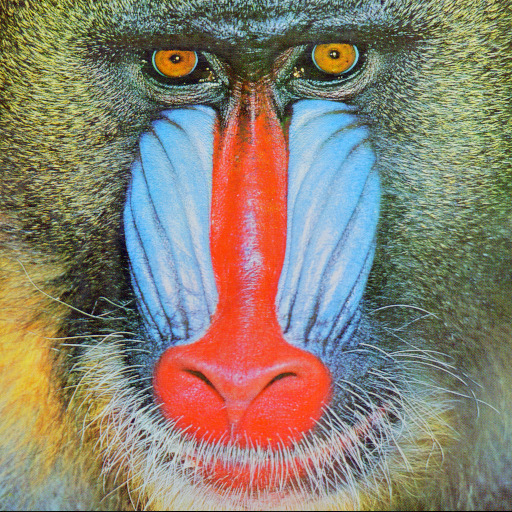
\includegraphics{images/mandrill.jpg}
\caption{The ``Mandrill'' standard test image, sometimes erroneously
called ``Baboon'', is a popular sample photo and used in image
processing research.}\label{fig:mandrill}
\end{figure}

\subsubsection{Citations}\label{citations}

Bibliographic data should be collected in a file \texttt{paper.bib}; it
should be formatted in the BibLaTeX format, although plain BibTeX is
acceptable as well. All major citation managers offer to export these
formats.

Cite a bibliography entry by referencing its identifier:
\texttt{{[}@upper1974{]}} will create the reference
``(\citeproc{ref-upper1974}{Upper, 1974})''. Omit the brackets when
referring to the author as part of a sentence: ``For a case study on
writers block, see Upper (\citeproc{ref-upper1974}{1974}).'' Please
refer to the
\href{https://pandoc.org/MANUAL\#extension-citations}{pandoc manual} for
additional features, including page locators, prefixes, suffixes, and
suppression of author names in citations.

\subsubsection{Mathematical Formulæ}\label{mathematical-formuluxe6}

Equations and other math content has is marked by dollar signs
(\texttt{\$}). A single dollar sign should be used for math that will
appear directly within the text, and \texttt{\$\$} should be used when
the formula is to be presented in ``display'' style, i.e., centered and
on a separate line. The formula itself must be given using TeX syntax.

To give some examples: When discussing a variable \(x\) or a short
formula like \(\sin \frac{\pi}{2}\), we would write \texttt{\$x\$} and
\texttt{\$\textbackslash{}sin\ \textbackslash{}frac\{\textbackslash{}pi\}\{2\}\$},
respectively. However, for more complex formulæ, display style is more
appropriate. Writing
\texttt{\$\$\textbackslash{}int\_\{-\textbackslash{}infty\}\^{}\{+\textbackslash{}infty\}\ e\^{}\{-x\^{}2\}\ \textbackslash{},\ dx\ =\ \textbackslash{}sqrt\{\textbackslash{}pi\}\$\$}
will give us

\[\int_{-\infty}^{+\infty} e^{-x^2} \, dx = \sqrt{\pi}\]

Numbered equations and internal cross-references are discussed
\hyperref[equations]{futher below}.

\subsubsection{Footnotes}\label{footnotes}

Syntax for footnotes centers around the ``caret'' character
\texttt{\^{}}. The symbol is also used as a delimiter for superscript
text and thereby mirrors the superscript numbers used to mark a footnote
in the final text.\footnote{Although it should be noted that some
  publishers prefer symbols or letters as footnote markers.}

\begin{Shaded}
\begin{Highlighting}[]
\NormalTok{Articles are published under a Creative Commons license}\OtherTok{[\^{}1]}\NormalTok{.}
\NormalTok{Software should use an OSI{-}approved license.}

\OtherTok{[\^{}1]: }\NormalTok{An open license that allows reuse.}
\end{Highlighting}
\end{Shaded}

Note numbers do not have to be sequential, they will be reordered
automatically in the publishing step. In fact, the identifier of a note
can be any sequence of characters, like \texttt{{[}\^{}marker{]}}, but
may not contain whitespace characters.

The above example results in the following output:

\begin{quote}
Articles are published under a Creative Commons license\footnote{An open
  license that allows reuse.}. Software should use an OSI-approved
license.
\end{quote}

\subsection{Blocks}\label{blocks}

The larger components of a document are called ``blocks''.

\subsubsection{Headings}\label{headings}

Headings are added with \texttt{\#} followed by a space, where each
additional \texttt{\#} demotes the heading to a level lower in the
hierarchy:

\begin{Shaded}
\begin{Highlighting}[]
\FunctionTok{\# Section}

\FunctionTok{\#\# Subsection}

\FunctionTok{\#\#\# Subsubsection}
\end{Highlighting}
\end{Shaded}

Please start headings on the first level. The maximum supported level is
5, but paper authors should usually try to limit themselves to headings
of the first two or three levels.

\paragraph{Deeper nesting}\label{deeper-nesting}

Forth- and fifth-level subsections -- like this one and the following
heading -- are supported by the system; however, their use is
discouraged.

\subparagraph{Avoiding excessive
nesting}\label{avoiding-excessive-nesting}

Usually \hyperref[lists]{lists}, as described in the next section,
should be preferred over forth- and fifth-level headings.

\subsubsection{Lists}\label{lists}

Bullet lists and numbered lists, a.k.a. enumerations, offer an
additional method to present sequential and hierarchical information.

\begin{Shaded}
\begin{Highlighting}[]
\SpecialStringTok{{-} }\NormalTok{apples}
\SpecialStringTok{{-} }\NormalTok{citrus fruits}
\SpecialStringTok{  {-} }\NormalTok{lemons}
\SpecialStringTok{  {-} }\NormalTok{oranges}
\end{Highlighting}
\end{Shaded}

\begin{itemize}
\tightlist
\item
  apples
\item
  citrus fruits

  \begin{itemize}
  \tightlist
  \item
    lemons
  \item
    oranges
  \end{itemize}
\end{itemize}

Enumerations start with the number of the first item. Using the the
first two
\href{https://en.wikipedia.org/wiki/Laws_of_thermodynamics}{laws of
thermodynamics} as example.

\begin{Shaded}
\begin{Highlighting}[]
\SpecialStringTok{0. }\NormalTok{If two systems are each in thermal equilibrium with a third, they are}
\NormalTok{   also in thermal equilibrium with each other.}
\SpecialStringTok{1. }\NormalTok{In a process without transfer of matter, the change in internal}
\NormalTok{   energy, $\textbackslash{}Delta U$, of a thermodynamic system is equal to the energy}
\NormalTok{   gained as heat, $Q$, less the thermodynamic work, $W$, done by the}
\NormalTok{   system on its surroundings. $$\textbackslash{}Delta U = Q {-} W$$}
\end{Highlighting}
\end{Shaded}

Rendered:

\begin{enumerate}
\def\labelenumi{\arabic{enumi}.}
\setcounter{enumi}{-1}
\tightlist
\item
  If two systems are each in thermal equilibrium with a third, they are
  also in thermal equilibrium with each other.
\item
  In a process without transfer of matter, the change in internal
  energy, \(\Delta U\), of a thermodynamic system is equal to the energy
  gained as heat, \(Q\), less the thermodynamic work, \(W\), done by the
  system on its surroundings. \[\Delta U = Q - W\]
\end{enumerate}

\section{Article metadata}\label{article-metadata}

\subsection{Names}\label{names}

Providing an author name is straight-forward: just set the \texttt{name}
attribute. However, sometimes fine-grained control over the name is
required.

\subsubsection{Name parts}\label{name-parts}

There are many ways to describe the parts of names; we support the
following:

\begin{itemize}
\tightlist
\item
  given names,
\item
  surname,
\item
  dropping particle,
\item
  non-dropping particle,
\item
  and suffix.
\end{itemize}

We use a heuristic to parse names into these components. This parsing
may produce the wrong result, in which case it is necessary to provide
the relevant parts explicitly.

The respective field names are

\begin{itemize}
\tightlist
\item
  \texttt{given-names} (aliases: \texttt{given}, \texttt{first},
  \texttt{firstname})
\item
  \texttt{surname} (aliases: \texttt{family})
\item
  \texttt{suffix}
\end{itemize}

The full display name will be constructed from these parts, unless the
\texttt{name} attribute is given as well.

\subsubsection{Particles}\label{particles}

It's usually enough to place particles like ``van'', ``von'', ``della'',
etc. at the end of the given name or at the beginning of the surname,
depending on the details of how the name is used.

\begin{itemize}
\tightlist
\item
  \texttt{dropping-particle}
\item
  \texttt{non-dropping-particle}
\end{itemize}

\subsubsection{Literal names}\label{literal-names}

The automatic construction of the full name from parts is geared towards
common Western names. It may therefore be necessary sometimes to provide
the display name explicitly. This is possible by setting the
\texttt{literal} field, e.g., \texttt{literal:\ Tachibana\ Taki}. This
feature should only be used as a last resort.

\subsubsection{Example}\label{example}

\begin{Shaded}
\begin{Highlighting}[]
\FunctionTok{authors}\KeywordTok{:}
\AttributeTok{  }\KeywordTok{{-}}\AttributeTok{ }\FunctionTok{name}\KeywordTok{:}\AttributeTok{ John Doe}
\AttributeTok{    }\FunctionTok{affiliation}\KeywordTok{:}\AttributeTok{ }\StringTok{\textquotesingle{}1\textquotesingle{}}

\AttributeTok{  }\KeywordTok{{-}}\AttributeTok{ }\FunctionTok{given{-}names}\KeywordTok{:}\AttributeTok{ Ludwig}
\AttributeTok{    }\FunctionTok{dropping{-}particle}\KeywordTok{:}\AttributeTok{ van}
\AttributeTok{    }\FunctionTok{surname}\KeywordTok{:}\AttributeTok{ Beethoven}
\AttributeTok{    }\FunctionTok{affiliation}\KeywordTok{:}\AttributeTok{ }\StringTok{\textquotesingle{}3\textquotesingle{}}

\CommentTok{  \# not recommended, but common aliases can be used for name parts.}
\AttributeTok{  }\KeywordTok{{-}}\AttributeTok{ }\FunctionTok{given}\KeywordTok{:}\AttributeTok{ Louis}
\AttributeTok{    }\FunctionTok{non{-}dropping{-}particle}\KeywordTok{:}\AttributeTok{ de}
\AttributeTok{    }\FunctionTok{family}\KeywordTok{:}\AttributeTok{ Broglie}
\AttributeTok{    }\FunctionTok{affiliation}\KeywordTok{:}\AttributeTok{ }\StringTok{\textquotesingle{}4\textquotesingle{}}
\end{Highlighting}
\end{Shaded}

The name parts can also be collected under the author's \texttt{name}:

\begin{Shaded}
\begin{Highlighting}[]
\FunctionTok{authors}\KeywordTok{:}
\AttributeTok{  }\KeywordTok{{-}}\AttributeTok{ }\FunctionTok{name}\KeywordTok{:}
\AttributeTok{      }\FunctionTok{given{-}names}\KeywordTok{:}\AttributeTok{ Kari}
\AttributeTok{      }\FunctionTok{surname}\KeywordTok{:}\AttributeTok{ Nordmann}
\end{Highlighting}
\end{Shaded}

\subsection{Affiliations}\label{affiliations}

Each affiliation requires an \texttt{index} and \texttt{name}.

Optionally, the Research Organization Registry (ROR) identifier for the
top-level organization can be annotated with the \texttt{ror} key. Note
that ROR does not include departments in its
\href{https://ror.org/registry/\#scope-and-criteria-for-inclusion}{scope},
so ROR annotations are typically made to the top-level organization.

\begin{Shaded}
\begin{Highlighting}[]
\FunctionTok{authors}\KeywordTok{:}
\AttributeTok{  }\KeywordTok{{-}}\AttributeTok{ }\FunctionTok{name}\KeywordTok{:}\AttributeTok{ Albert Krewinkel}
\AttributeTok{    }\FunctionTok{affiliation}\KeywordTok{:}\AttributeTok{ }\KeywordTok{[}\AttributeTok{ }\DecValTok{1}\KeywordTok{,}\AttributeTok{ }\DecValTok{2}\KeywordTok{,}\AttributeTok{ }\DecValTok{3}\AttributeTok{ }\KeywordTok{]}

\FunctionTok{affiliations}\KeywordTok{:}
\AttributeTok{  }\KeywordTok{{-}}\AttributeTok{ }\FunctionTok{index}\KeywordTok{:}\AttributeTok{ }\DecValTok{1}
\AttributeTok{    }\FunctionTok{name}\KeywordTok{:}\AttributeTok{ Open Journals}
\AttributeTok{  }\KeywordTok{{-}}\AttributeTok{ }\FunctionTok{index}\KeywordTok{:}\AttributeTok{ }\DecValTok{2}
\AttributeTok{    }\FunctionTok{name}\KeywordTok{:}\AttributeTok{ Pandoc Development Team}
\AttributeTok{  }\KeywordTok{{-}}\AttributeTok{ }\FunctionTok{index}\KeywordTok{:}\AttributeTok{ }\DecValTok{3}
\AttributeTok{    }\FunctionTok{name}\KeywordTok{:}\AttributeTok{ Technische Universitaet Hamburg}
\AttributeTok{    }\FunctionTok{ror}\KeywordTok{:}\AttributeTok{ 04bs1pb34}
\end{Highlighting}
\end{Shaded}

\section{Internal references}\label{internal-references}

Markdown has no default mechanism to handle document internal
references, often called ``cross-references''. This conflicts with goal
of \href{https://theoj.org}{Open Journals} is to provide authors with a
seamless and pleasant writing experience. This includes convenient
cross-reference generation, which is why a limited set of LaTeX commands
are supported. In a nutshell, elements that were marked with
\texttt{\textbackslash{}label} and can be referenced with
\texttt{\textbackslash{}ref} and \texttt{\textbackslash{}autoref}.

\begin{figure}
\centering
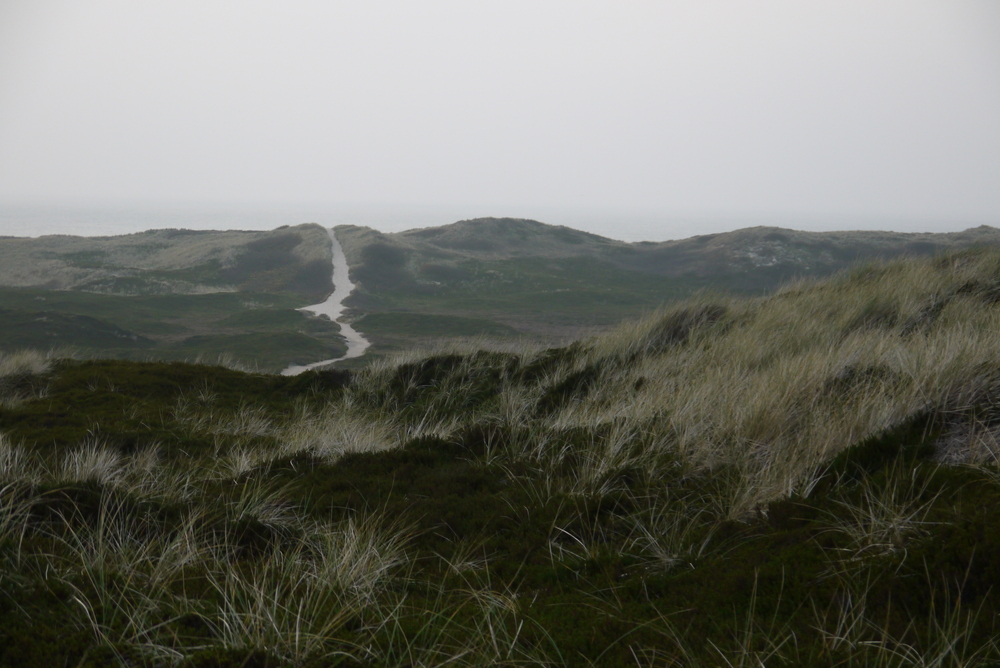
\includegraphics[width=1\textwidth,height=\textheight]{images/sylt.jpg}
\caption{View of coastal dunes in a nature reserve on Sylt, an island in
the North Sea. Sylt (Danish: \emph{Slid}) is Germany's northernmost
island.}\label{sylt}
\end{figure}

\subsection{Tables and figures}\label{tables-and-figures}

Tables and figures can be referenced if they are given a \emph{label} in
the caption. In pure Markdown, this can be done by adding an empty span
\texttt{{[}{]}\{label="floatlabel"\}} to the caption. LaTeX syntax is
supported as well: \texttt{\textbackslash{}label\{floatlabel\}}.

Link to a float element, i.e., a table or figure, with
\texttt{\textbackslash{}ref\{identifier\}} or
\texttt{\textbackslash{}autoref\{identifier\}}, where
\texttt{identifier} must be defined in the float's caption. The former
command results in just the float's number, while the latter inserts the
type and number of the referenced float. E.g., in this document
\texttt{\textbackslash{}autoref\{proglangs\}} yields
``\autoref{proglangs}'', while \texttt{\textbackslash{}ref\{proglangs\}}
gives ``\ref{proglangs}''.

\begin{longtable}[]{@{}
  >{\raggedright\arraybackslash}p{(\columnwidth - 8\tabcolsep) * \real{0.1493}}
  >{\centering\arraybackslash}p{(\columnwidth - 8\tabcolsep) * \real{0.2537}}
  >{\centering\arraybackslash}p{(\columnwidth - 8\tabcolsep) * \real{0.2836}}
  >{\raggedright\arraybackslash}p{(\columnwidth - 8\tabcolsep) * \real{0.1791}}
  >{\raggedright\arraybackslash}p{(\columnwidth - 8\tabcolsep) * \real{0.1343}}@{}}
\caption{Comparison of programming languages used in the publishing
tool. {}}\tabularnewline
\toprule\noalign{}
\begin{minipage}[b]{\linewidth}\raggedright
Language
\end{minipage} & \begin{minipage}[b]{\linewidth}\centering
Typing
\end{minipage} & \begin{minipage}[b]{\linewidth}\centering
Garbage Collected
\end{minipage} & \begin{minipage}[b]{\linewidth}\raggedright
Evaluation
\end{minipage} & \begin{minipage}[b]{\linewidth}\raggedright
Created
\end{minipage} \\
\midrule\noalign{}
\endfirsthead
\toprule\noalign{}
\begin{minipage}[b]{\linewidth}\raggedright
Language
\end{minipage} & \begin{minipage}[b]{\linewidth}\centering
Typing
\end{minipage} & \begin{minipage}[b]{\linewidth}\centering
Garbage Collected
\end{minipage} & \begin{minipage}[b]{\linewidth}\raggedright
Evaluation
\end{minipage} & \begin{minipage}[b]{\linewidth}\raggedright
Created
\end{minipage} \\
\midrule\noalign{}
\endhead
\bottomrule\noalign{}
\endlastfoot
Haskell & static, strong & yes & non-strict & 1990 \\
Lua & dynamic, strong & yes & strict & 1993 \\
C & static, weak & no & strict & 1972 \\
\end{longtable}

\subsection{Equations}\label{equations}

Cross-references to equations work similar to those for floating
elements. The difference is that, since captions are not supported for
equations, the label must be included in the equation:

\begin{verbatim}
$$a^n + b^n = c^n \label{fermat}$$
\end{verbatim}

Referencing, however, is identical, with
\texttt{\textbackslash{}autoref\{eq:fermat\}} resulting in
``\autoref{eq:fermat}''.

\[a^n + b^n = c^n \label{eq:fermat}\]

Authors who do not wish to include the label directly in the formula can
use a Markdown span to add the label:

\begin{verbatim}
[$$a^n + b^n = c^n$$]{label="eq:fermat"}
\end{verbatim}

\section{Behind the scenes}\label{behind-the-scenes}

Readers may wonder about the reasons behind some of the choices made for
paper writing. Most often, the decisions were driven by radical
pragmatism. For example, Markdown is not only nearly ubiquitous in the
realms of software, but it can also be converted into many different
output formats. The archiving standard for scientific articles is JATS,
and the most popular publishing format is PDF. Open Journals has built
its pipeline based on \href{https://pandoc.org}{pandoc}, a universal
document converter that can produce both of these publishing formats --
and many more.

A common method for PDF generation is to go via LaTeX. However, support
for tagging -- a requirement for accessible PDFs -- is not readily
available for LaTeX. The current method used ConTeXt, to produce tagged
PDF/A-3, a format suited for archiving
(\citeproc{ref-pdfa3}{\emph{Document Management -- Electronic Document
File Format for Long-Term Preservation -- Part 3}, 2012}).

\phantomsection\label{refs}
\begin{CSLReferences}{1}{0.5}
\bibitem[\citeproctext]{ref-pdfa3}
\emph{Document management -- electronic document file format for
long-term preservation -- part 3: Use of {ISO} 32000-1 with support for
embedded files ({PDF/A-3})}. (2012). {[}Standard{]}. International
Organization for Standardization.

\bibitem[\citeproctext]{ref-krewinkel2017}
Krewinkel, A., \& Winkler, R. (2017). Formatting open science: Agilely
creating multiple document formats for academic manuscripts with pandoc
scholar. \emph{PeerJ Computer Science}, \emph{3}, e112.
\url{https://doi.org/10.7717/peerj-cs.112}

\bibitem[\citeproctext]{ref-smith2018}
Smith, A. M., Niemeyer, K. E., Katz, D. S., Barba, L. A., Githinji, G.,
Gymrek, M., Huff, K. D., Madan, C. R., Cabunoc Mayes, A., Moerman, K.
M., Prins, P., Ram, K., Rokem, A., Teal, T. K., Valls Guimera, R., \&
Vanderplas, J. T. (2018). Journal of open source software (JOSS): Design
and first-year review. \emph{PeerJ Computer Science}, \emph{4}, e147.
\url{https://doi.org/10.7717/peerj-cs.147}

\bibitem[\citeproctext]{ref-yaml_website}
\emph{The {Official YAML Web Site}}. (2022, April 19).
\url{https://yaml.org/}

\bibitem[\citeproctext]{ref-upper1974}
Upper, D. (1974). The unsuccessful self-treatment of a case of "writer's
block". \emph{Journal of Applied Behavior Analysis}, \emph{7}(3), 497.
\url{https://doi.org/10.1901/jaba.1974.7-497a}

\end{CSLReferences}

\end{document}
